\documentclass[9pt, compress]{beamer}
\usetheme[titleprogressbar]{m}

\usepackage[scale=2]{ccicons}
\usepackage{minted}
\usepackage{booktabs}
\usepackage{multirow}
\usepackage{amsmath}
\usepackage{arydshln}
\usepackage{amssymb}
\usepgfplotslibrary{dateplot}
\usepackage{booktabs,caption,fixltx2e}
\usepackage[flushleft]{threeparttable}
\usepackage{color}


\usepackage{tikz}
\usepackage{verbatim}
\usetikzlibrary{arrows,positioning,calc} 
\usepackage{relsize}
\newcommand\LM{\ensuremath{\mathit{LM}}}
\newcommand\IS{\ensuremath{\mathit{IS}}}

\tikzset{
    %Define standard arrow tip
    >=stealth',
    %Define style for boxes
    punkt/.style={
           rectangle,
           rounded corners,
           draw=black, very thick,
           text width=6.5em,
           minimum height=2em,
           text centered},
    % Define arrow style
    pil/.style={
           <-,
           thick,
           shorten <=2pt,
           shorten >=2pt,},
    % Node for explanation       
    punk/.style={
           rectangle,
           draw=white, thin,
           text width=17em,
           minimum height=2em,
           text centered}   
}
\usepackage{pgfplots}

\author{Syngjoo Choi (SNU), Booyuel Kim (KDIS), Minseon Park (KDI), Yoonsoo Park (KDI), and Euncheol Shin (KHU)} 
\title{Rationality, Preference Aggregation and Pareto Efficiency of Group Decision Under Risk}
%\subtitle{}
%\logo{}
%\institute{\textbf{KDI}}
\date{June 23th, 2017}
%\subject{}
%\setbeamercovered{transparent}
%\setbeamertemplate{navigation symbols}{}
\begin{document}
	\maketitle
    \begin{frame}\frametitle{Introduction}
	\begin{itemize}
    \item We make many types of collective decision in our daily life
    \begin{itemize}
    \item Household's decision on consumption and saving, a firm's resource allocation among projects, decision on tax and transfer in legislature
    \end{itemize}
    \item Previous studies have focused on preference aggregation (Baillon et al. (2016), Bateman and Munro (2005), Palma et al. (2010)) or inconsistency of group decision from preference conflict (Arrow (1951), Browning and Chiappori (1998), Chiappori and Ekeland (2011), Bourguignon et al. (2009))
    \end{itemize}
    \end{frame}
   
    \begin{frame}\frametitle{Fundamental Questions on Group Decision}
    Three fundamental questions on group decision
    \begin{block}{1. Rationality Extension:}
    If each individual's choices are consistent with the utility maximization model, do a group's choices also tend to be? 
    \end{block}
    \begin{block}{2. Risk Preference Aggregation:}
    Are individuals' risk preferences reflected into that of a group?
    \end{block}
    \begin{block}{3. Pareto Efficiency:}
    Are a group's choices Pareto efficient? Is it maximizing social welfare?
    \end{block}
	\end{frame}
    
	\begin{frame}\frametitle{Contribution}
    \begin{enumerate}    
    \item The first study answers for the three fundamental questions on group decision, using a unique experimental design and a large sample (N=1572) 
    \item We devise novel ways to test Pareto efficiency given individual and collective choice data on a budget line, and compute the severity of inefficiency from Pareto inefficient choices
    \item Taking the revealed preference approach, we show the relationship between individual and group rationality
    \end{enumerate}
    \end{frame}
    
    \begin{frame}\frametitle{Preview for Results}
    Our main results are
    \begin{enumerate}
    \item Individual rationality extends to that of group
    \item Individual risk preference (both probability weighting type (RDU or EUT) and risk aversion) is strongly reflected into that of group
    \item Many joint decisions are close to be Pareto efficient. In addition, Pareto efficiency is positively correlated with collective rationality
    \end{enumerate}
    \end{frame}
    
    \begin{frame}\frametitle{Experimental Design\footnote{Basically it is based on Choi et al. (2007)} and Procedures}
    \label{decision}
        \begin{itemize}
        \item A subject chooses the menu of the outcome $(x_1,x_2)$ of a lottery $L=(x_1,x_2;0.5,0.5)$ on a given budget line $p_1x_1+p_2x_2=1$
\begin{figure}
        \includegraphics[width=160pt,height=120pt]{img/screen.png}
		\end{figure}
    \item 18 times of individual decisions $\Rightarrow$ 18 times of collective decisions (free conversation, random matching within a class)
    \item Each one of individual and collective choices is randomly selected to be reimbursed
    \end{itemize}
        \end{frame}
        
        \begin{frame} \frametitle{Extension: Testing Collective Rationality}
        \begin{itemize}
        \item Revealed preference approach : tests consistency within choices (Generalized Axiom of Revealed Preference (GARP))
        \item CCEI (Afriat (1972))\footnote{We also use Varian (1991) for robustness check, and all results are preserved qualitatively} : 1-CCEI  stands for how much of budget should be removed to rationalize inconsistent choices with the utility maximization model
        \item CCEI$\in[0,1]$, and the bigger it is, the less severe the violation is 
        \end{itemize}
        \end{frame}
        
        \begin{frame} \frametitle{Extension: Individual Rationality Leads to Group Rationality}
        \begin{figure}
        \includegraphics[width=200pt,height=150pt]{img/Figure4.png}
        \caption{CDFs of Collective CCEI by Individual Rationality}
		\end{figure}
        \begin{small}
        \begin{itemize}
        \item 57.8\%, 64.9\% and 80.9\% of neither,either,both-rational pairs have CCEI$\geq$ 0.9\footnote{This result is robust to the cutoff of CCEI - 0.95 and 0.99.}
        \end{itemize}
        \end{small}
	\end{frame}

       \begin{frame}\frametitle{Preference Aggregation: Using a Parametric Measure}    
    \label{alpha}
        \begin{itemize}   
         \item $U(x_{min},x_{max})=\alpha{u(x_{min})}+(1-\alpha)u(x_{max})$ \footnote{In addition, we assume CARA utility function which takes the specific form $u(x)=-\frac{exp(-\rho x)}{\rho}$} (Gul (1991))
     	\item  If $\alpha=\frac{1}{2}$, \textbf{Expected Utility Form (EUT)}. If $\alpha>\frac{1}{2}$, then one said to show disappointment aversion; $\alpha<\frac{1}{2}$, elation loving. Altogether, \textbf{Rank Dependent Utility Form (RDU)} \footnote{In our data, 20.2\%, 29.3\% of individuals and pairs follow RDU, respectively. We define a utility function follows EUT if $0.5 \in 95\%$ of $\alpha$ using bootstrapped standard error}
        \end{itemize}
      \begin{table}[]
\centering
\begin{tabular}{@{}ccllll@{}}
\toprule 
\multicolumn{2}{l}{Individual} & \multicolumn{1}{c}{Both EUT} & \multicolumn{1}{c}{EUT and RDU} & \multicolumn{1}{c}{Both RDU} & Total \\ \cmidrule(r){1-6}
\multirow{2}{*}{Collective} & EUT & 74.5(117) & 59.1(52) & 50.0(7) & 68.0(176) \\
	& RDU & 25.5(40) & 40.1(36) & 50.0(7) & 32.1(83) \\
	& Total & 100(157) & 100(88) & 100(14) & 100(259) \\ \bottomrule
    \multicolumn{6}{l}{\footnotesize{EUT is defined as 0.5$\in$ 95\% CI of $\alpha$, N for each case in parenthesis}} \\
     \multicolumn{6}{l}{\footnotesize{Only includes pairs with both individuals' and collective CCEI>=0.9}}
\end{tabular}
\caption{Percentage of RDU Type of Pairs by Individual Type}
\end{table}
    \hyperlink{RDU}{\beamergotobutton{RDU}} \hyperlink{ex}{\beamergotobutton{ex}}
    \hyperlink{estimation}{\beamerreturnbutton{est}}
    \end{frame}
         
      \begin{frame}\frametitle{Preference Aggregation: Using a Non-parametric Measure}
    \label{Risk}
    \begin{itemize}
    \item We use $\Sigma_{j=1}^{18} \frac{x_{cheaper}}{x_1+x_2} \in [0.5,1]$ which is between $(0.5,1)$, and the bigger it is, the less risk averse the preference is \footnote{Mean(sd) of individual/collective game=0.67(0.13)/0.70(0.13)} 
    \end{itemize}
        \begin{figure}
        \includegraphics[width=200pt,height=150pt]{img/Figure5.png}
        \caption{CDFs of Collective Risk Preference by Individual Risk Attitude}\footnote{20.7\%, 49.2\% and 73.7\% of neither,either,both-risk averse pairs are more risk averse than the mean}
		\end{figure}
   \end{frame}
    
	 \begin{frame}\frametitle{Pareto Efficiency: Measure}
       	 \begin{block}{Pareto Efficiency:}
         A pair's choice $X_c$ is \textbf{Pareto efficient} if and only if it is between $X^*_1=argmax_{(x_1,x_2)}\hat{U}_1(x_1,x_2)$ and $X^*_2=argmax_{(x_1,x_2)}\hat{U}_2(x_1,x_2)$\footnote{The condition holds as long as utility function is monotone and symmetric. We say a utility function is symmetric if $U(x_1,x_2)=U(x_2,x_1)$}
         \end{block}
\begin{center}        
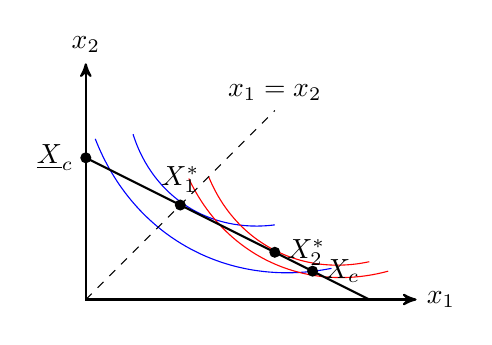
\begin{tikzpicture}[
        scale=1.2,
        IS/.style={black, thick},
        LM/.style={black, dashed},
        i1/.style={blue},
        i2/.style={red},
        axis/.style={thick, ->, >=stealth', line join=miter},
        every node/.style={color=black},
        dot/.style={circle,fill=black,minimum size=4pt,inner sep=0pt,
            outer sep=-1pt},
    ]
    % axis
    \draw[axis,<->] (3.5,0) node(xline)[right] {$x_1$} -|
                    (0,2.5) node(yline)[above] {$x_2$};
    % IS-LM diagram
    \draw[i1] (0.5,1.75) to [bend right=40] coordinate[pos=0.1] (l_i) (2,0.79) ;
    \draw[i1] (0.1,1.7) to [bend right=40] coordinate[pos=0.1] (l_i) (2.6,0.33) ;
    \draw[i2] (1.3,1.3) to [bend right=40] coordinate[pos=0.1] (l_i) (3,0.4) ;
    \draw[i2] (1.09,1.28) to [bend right=40] coordinate[pos=0.1] (l_i) (3.2,0.3) ;
    \draw[LM] (0,0) coordinate (LM_1) -- (2,2) coordinate (LM_2) node[above] {$x_1=x_2$};
    \draw[IS] (0,1.5) coordinate (IS_1) -- (3,0) coordinate (IS_2) ;

    %Intersection is calculated "manually" since Tikz does not offer
    %intersection calculation for parabolas
    \node[dot,label=above:$X^*_1$] at (1,1) (int1) {};
	\node[dot,label=right:$X^*_2$] at (2,0.5) (int1) {};
	\node[dot,label=right:$X_c$] at (2.4,0.3) (int1) {};
    \node[dot,label=left:$\underline{X}_c$] at (0,1.5) (int1) {};    
    \end{tikzpicture}
\end{center}
    \end{frame}
    
	 \begin{frame}\frametitle{Pareto Efficiency: Continuous Measure}
       	 \begin{block}{Utility Loss from Pareto Inefficient Choice:=}
         \begin{center} 
         \begin{equation}
         \frac{1}{18}\Sigma_{j=1}^{18}\frac{1}{2}\Sigma_{i=1}^2\frac{u_i(\bar{X}_{cj})-u_i(X_{cj})}{u_i(\bar{X}_{cj})-u_i(\underline{X}_{ij})} \in[0,1]
          \end{equation} 
          \end{center}
         where $X_c$: collective choice, $\underline{X}$: worst choice on the budget line. $j$ denote the sequence of budget lines and $i$ individuals. Finally, $\bar{X}=argmin(d(X_c,X)), X\in \lbrace X|u_i(X)>=u_i(X_c) \rbrace$ with strict inequality for one $i$. If such $X$ does not exist, $\bar{X}=X_c$
         \end{block}
    \end{frame}
    
    \begin{frame}\frametitle{Pareto Efficiency: Results}
    \begin{figure}       
     \includegraphics[width=200pt,height=150pt]{img/Figure8.png}
     \caption{Distribution of the Utility Loss from Pareto Inefficiency By Pairs}
		\end{figure}   
        \begin{itemize}
        \item The mean(sd) of utility loss is 0.09(0.12) when only including pairs with both individuals' CCEI>0.9 
        \end{itemize}
    \end{frame}
    
    \begin{frame}\frametitle{Pareto Efficiency: Results}
    \begin{figure}       
     \includegraphics[width=200pt,height=150pt]{img/Figure9.png}
               \caption{CDFs of the Utility Loss from Pareto Inefficient Choices by Collective Rationality}
		\end{figure}   
        \begin{itemize}
        \item Mean of utility loss for pairs with collective CCEI>0.08 is 0.15. For CCEI<0.9, it is 0.15. This difference is statistically significant at 1\% significance level
        \end{itemize}
    \end{frame}
        
    \begin{frame}\frametitle{Conclusion}
    We study fundamental questions on group decision. And the results show
    \begin{block}{Rationality Extension}
   Individual rationality extends to that of a group
    \end{block}
    \begin{block}{Preference Aggregation}
    Individuals' risk attitude is strongly reflected into that of group
    \end{block}
    \begin{block}{Pareto Efficiency}
    There exists remarkable heterogeneity across groups' loss from Pareto inefficient choices. Much of such variation is resulted from collective rationality
    \end{block}
    \end{frame}
    
 
    
 	\begin{frame}\frametitle{Previous Literature}
    \begin{scriptsize}
    \begin{table}[]
\centering
\begin{tabular}{@{}lll@{}}
\toprule
Groups & Main Focus & Literature \\ \midrule
\begin{tabular}[c]{@{}l@{}}Experimental studies \\ on the  comparison between \\ individual and group   decision\end{tabular} & \begin{tabular}[c]{@{}l@{}}Which one is closer \\ to the theoretical prediction\end{tabular} & \begin{tabular}[c]{@{}l@{}}Bone et al. (1999), \\ Cason and Mui(1997), \\ Charness  et al. (2007), \\ Charness and Sutter (2012), \\ Cooper and Kagel (2005), \\ Carbone   et al. (2016), \\ Kerr at el. (1996),  Kugler et al. (2012), \\ Masclet et al.(2009), \\ Shupp and Williams (2008), \\ Sutter (2009)\end{tabular} \\ \hline
\begin{tabular}[c]{@{}l@{}}Experimental studies \\ on preference aggregation \end{tabular} & \begin{tabular}[c]{@{}l@{}} How risk attitude/ \\ time preference is aggregated \end{tabular} & \begin{tabular}[c]{@{}l@{}}Abdellaoui et al. (2010), \\ Baillon et al. (2016),\\  Bateman and Munro (2005),\\   Palma et al. (2010), \\ Lee at el. (2012)\end{tabular}\\ \hline
\begin{tabular}[c]{@{}l@{}}Empirical studies \\ on household resource  allocation\end{tabular} & \begin{tabular}[c]{@{}l@{}}Test representative agent \\ model \\   Factors for bargaining power\end{tabular} & \begin{tabular}[c]{@{}l@{}}Browning and Chiappori (1998), \\ Chiappori and  Ekeland (2011), \\ Friedberg and Webb (2006), \\ Bourguignon et al. (2009)\end{tabular} \\ \hline
Theoretical studies \\ on preference aggregation & \begin{tabular}[c]{@{}l@{}}Representative agent models\\   Impossibility theorem\end{tabular} & Arrow, Jackson and Yariv (2014)  \\ \bottomrule
\end{tabular}
\end{table}
\end{scriptsize}
    \end{frame}
    
    
	\begin{frame}{Experimental Design and Procedures}
    \label{Design}
    \begin{center}
	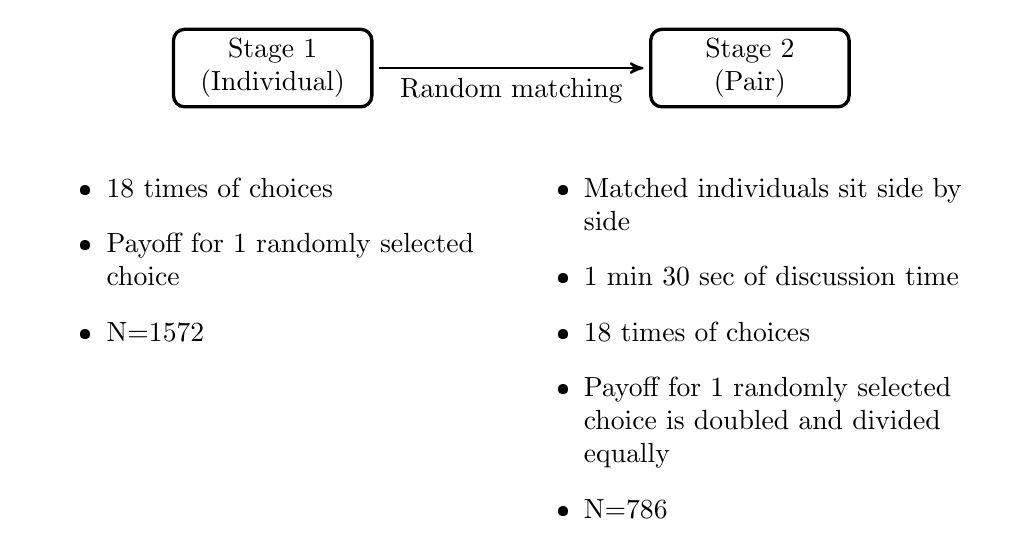
\begin{tikzpicture}[node distance=1cm, auto,]
    	\node[punkt] (stage1) {Stage 1 (Individual)} ;
    	\node[punkt, right=3.5cm of stage1] (stage2) {Stage 2 \\ (Pair)}
  		edge[pil] node[auto] {Random matching}(stage1);
    	\node[punk, below=0.3cm of stage1] (indiv) 
    	{\begin{itemize}
    	\item 18 times of choices
    	\item Payoff for 1 randomly selected choice
        \item N=1572
    	\end{itemize}} ;
       \node[punk, below=0.3cm of stage2] (col) 
       {\begin{itemize}
       \item Matched individuals sit side by side
       \item 1 min 30 sec of discussion time 
       \item 18 times of choices 
       \item Payoff for 1 randomly selected choice is doubled and divided equally 
       \item N=786
       \end{itemize}} ;
	\end{tikzpicture}
    \begin{itemize}
    \item No feedback is given during the experiment and subjects are informed only the  sum of payoff from stage 1 and 2 after all the process
    \item The experiment is computerized using O-tree
    \hyperlink{ex}{\beamergotobutton{ex}}
    \end{itemize}
	\end{center}
	\end{frame}
    
     \begin{frame}\frametitle{Extension: Testing Rationality}
     \label{CCEI}
        \begin{block}{Generalized Axiom of Revealed Preference (GARP)}
         If $x^t$ is revealed preferred to $x^s$, then $x^s$ is not strictly revealed preferred to $x^t$ (\(p^sx^s \leq p^sx^t\))
        \end{block}
        \begin{block}{Afriat's theorem (Afriat (1967))}
		Observed choice data satisfy the GARP if and only if there exist a increasing, continuous and concave utility function that rationalize the observed choice. 
		\end{block}
        \begin{block}{Critical Cost Efficiency Index (CCEI(Afriat (1972)))}
		CCEI is the largest number \(e\in [0, 1]\) such that if $     e(p^1x^1)\geq p^1x^2, e(p^2x^2) \geq p^2x^3, ... , e(p^{n-1}x^{n-1}) \geq p^{n-1}x^n$, then $e(p^nx^n) \leq p^nx^1 $ \hyperlink{fig}{\beamergotobutton{fig}}       
        \end{block}
        In our data, 62.6\%(50.7\%) of individuals' CCEI are equal to or greater than 0.90(0.95). On pairs, the percentage is 70.4\%(60\%) \\
        \hyperlink{ex}{\beamergotobutton{ex}}         
    \end{frame}
    
            \begin{frame} \frametitle{Extension: Measure of Rationality}
        \label{fig}
        \begin{figure}
        \includegraphics[width=200pt,height=150pt]{img/fig_ccei.png}
		\end{figure}
        \hyperlink{CCEI}{\beamergotobutton{CCEI}}
        \end{frame}
            
        \begin{frame}\frametitle{Example of Individual-pair Relative Demand Curve}
    \label{ex}
    \begin{figure}       
        \includegraphics[width=270pt,height=180pt]{img/relconsumption284.png}
       \end{figure}   
    \hyperlink{Design}{\beamerreturnbutton{Design}}
    \hyperlink{CCEI}{\beamerreturnbutton{CCEI}}
    \hyperlink{alpha}{\beamerreturnbutton{alpha}}   
    \hyperlink{Risk}{\beamerreturnbutton{Risk}}
    \end{frame}

        \begin{frame}\frametitle{Example of Individual-pair Relative Demand Curve}
    \begin{figure}       
        \includegraphics[width=270pt,height=180pt]{img/relconsumption623.png}
       \end{figure}   
    \hyperlink{Design}{\beamerreturnbutton{Design}}
    \hyperlink{CCEI}{\beamerreturnbutton{CCEI}}
    \hyperlink{alpha}{\beamerreturnbutton{alpha}}   
    \hyperlink{Risk}{\beamerreturnbutton{Risk}}
    \end{frame}
    
  	\begin{frame}\frametitle{EUT and RDU}
        \label{RDU}
        \begin{figure}       
        \includegraphics[width=270pt,height=180pt]{img/indifcurve.png}
        \caption{Indifference Curve Depending on Probability Weighting}
		\end{figure}
        \hyperlink{alpha}{\beamerreturnbutton{alpha}}
   	\end{frame}
    
    \begin{frame}\frametitle{Estimation of Utility Function}
    \label{estimation}
    \begin{equation}
    (\hat{\alpha}, \hat{\rho})=argmin_{(\alpha,\rho)}\Sigma_{j=1}^{18}|\frac{x^*_{1j}(\alpha, \rho)}{x^*_{1j}(\alpha, \rho)+x^*_{2j}(\alpha, \rho)}-\frac{x_{1j}}{x_{1j}+x_{2j}}|
    \end{equation}
    where
    \begin{equation}
    (x^*_{1j}(\alpha, \rho),x^*_{2j}(\alpha, \rho))=argmax_{(x_{1j},x_{2j})}\alpha (-\frac{exp(-\rho x_{min})}{\rho})+(1-\alpha) (-\frac{exp(-\rho x_{max})}{\rho})
    \end{equation}
    given $p_{1j}x_{1j}+p_{2j}x_{2j}=1$ and $x_{min(max)}=min(max)(x_{1j},x_{2j})$
    \end{frame}
   
     \begin{frame}\frametitle{Preference Aggregation: Measuring Risk attitude}    
 \begin{block}{Parametric risk attitude: Risk Premium}
        \begin{itemize}   
         \item $U(x_{min},x_{max})=\alpha{u(x_{min})}+(1-\alpha)u(x_{max})$
     	 \item Risk premium $r(h=1)$: $U(w(1-r))=\alpha{U(w(1-h))}+(1-\alpha)U(w(1+h))$
        \item Mean(sd) of individual/collective game=0.15(0.96)/0.31(1.22)\footnote{CARA function assumed} \hyperlink{ex}{\beamergotobutton{ex}}
        \end{itemize}
    \end{block}    
    \end{frame}

       \begin{frame}\frametitle{Preference Attitude Aggregation: Result}
    \begin{figure}
        \includegraphics[width=200pt,height=150pt]{img/Figure6.png}
        \caption{CDFs of Collective Risk Premium by Individual Risk Attitude}
		\end{figure}
    \end{frame}

        \begin{frame}
    \begin{footnotesize}
    \begin{table}[]
\centering
\begin{tabular}{@{}lcccc@{}}
\toprule
Dependent Var. & \multicolumn{2}{c}{Collective Risk Preference} & \multicolumn{2}{c}{Collective Risk Premium} \\ 
 & (1) & (2) & (3) & (4) \\ \midrule
Ave.(Individual RP) & 0.811*** & 0.796*** &  &  \\
 & (0.060) & (0.062) &  &  \\
Dist.(Individual RPs) & 0.017 & 0.002 &  &  \\
 & (0.052) & (0.054) &  &  \\
Ave.(Individual Premium) &  &  & 0.277** & 0.242* \\
 &  &  & (0.127) & (0.135) \\
Dist.(Individual Premium) &  &  & 0.152* & 0.170** \\
 &  &  & (0.080) & (0.081) \\
Non coed &  & 0.017 &  & 0.064 \\
 &  & (0.010) &  & (0.091) \\
Two boys &  & 0.020 &  & 0.233 \\
 &  & (0.023) &  & (0.143) \\
Two girls &  & -0.021 &  & 0.296* \\
 &  & (0.015) &  & (0.167) \\
Math Score & No & Yes & No & Yes \\
Network Characteristics & No & Yes & No & Yes \\
TIPI Scores & No & Yes & No & Yes \\
Constant & 0.151*** & 0.065 & 0.157*** & 0.709 \\
 & (0.037) & (0.053) & (0.041) & (0.519) \\
Observations & 786 & 771 & 320 & 314 \\
R-squared & 0.318 & 0.341 & 0.068 & 0.133 \\ \midrule
\multicolumn{5}{l}{\begin{tabular}[c]{@{}l@{}}Notes: 1) *** p\textless0.01, **,p\textless0.05, * p\textless0.1,  2) Standard errors are clustered at class level\\         3) Network characteristics include mean, distance of indegree and  outdegree. \\ Dyadic relationship is also controlled., 4) TIPI scores consist of outgoing, \\ openness to experience, conscientiousness, emotional stability and agreeableness.\end{tabular}}
\end{tabular}
\end{table}
\end{footnotesize}
    \end{frame}


	\begin{frame}
    \begin{footnotesize}
    \begin{table}[]
\centering
\begin{tabular}{@{}lcccc@{}}
\toprule
Dependent Var. & \multicolumn{4}{c}{Utility Loss from Collective Decision} \\ \midrule
 & (1) & (2) & (3) & (4) \\
Collective CCEI & -0.369*** & -0.390*** & -0.365*** & -0.387*** \\
 & (0.067) & (0.058) & (0.066) & (0.056) \\
Ave.(Individual RP) & 0.093 & 0.099 &  &  \\
 & (0.114) & (0.101) &  &  \\
Dist.(Individual RP) & -0.139* & -0.129** &  &  \\
 & (0.072) & (0.062) &  &  \\
Ave.(Individual Premium) &  &  & -0.027 & -0.027* \\
 &  &  & (0.018) & (0.016) \\
Dist.(Individual Premium) &  &  & -0.002 & -0.006 \\
 &  &  & (0.010) & (0.009) \\
Non Coed &  & -0.011 &  & -0.009 \\
 &  & (0.023) &  & (0.023) \\
Two Boys &  & 0.065* &  & 0.072* \\
 &  & (0.039) &  & (0.039) \\
Two Girls &  & -0.018 &  & -0.014 \\
 &  & (0.027) &  & (0.026) \\
Constant & 0.413*** & 0.352** & 0.458*** & 0.400*** \\
 & (0.095) & (0.137) & (0.063) & (0.136) \\
Observations & 320 & 314 & 320 & 314 \\
R-squared & 0.075 & 0.220 & 0.070 & 0.219 \\ \midrule
\multicolumn{5}{l}{\begin{tabular}[c]{@{}l@{}}Notes: 1) *** p\textless0.01, **,p\textless0.05, * p\textless0.1,  2) Standard errors are clustered at class level\\         3) Network characteristics include mean, distance of indegree and  outdegree. \\ Dyadic relationship is also controlled., 4) TIPI scores consist of outgoing, \\ openness to experience, conscientiousness, emotional stability and agreeableness.\end{tabular}}
\end{tabular}
\end{table}
\end{footnotesize}
    \end{frame}
    
    \end{document}
    
    